\chapter{Alimentación y potencia}\label{cap:potencia}

\section{Dos fuentes separadas}

El robot tiene \textbf{dos fuentes de energía que nunca se tocan} (salvo el GND común):

\begin{description}
  \item[LiPo 3S para los motores] 11,1~V nominal (9,9--12,6~V), 8000~mAh (88,8~Wh). Alimenta los cinco IBT-2 y el
        buck de los servos. Los motores son de 12~V y el IBT-2 acepta de 5,5 a 27~V, así que la LiPo va
        \textbf{directa, sin convertidor}.
  \item[Power bank para la lógica] Xiaomi PB2030MI, 5~V 3~A por su cable USB-C. Alimenta la Raspberry Pi, y la Pi
        alimenta los dos ESP32 por USB.
\end{description}

\begin{idea}[Por qué separadas]
Un motor trabado puede pedir 10~A y hacer caer la tensión de la batería. Si la Pi estuviera en la misma batería,
se reiniciaría en medio de una cosecha. Con fuentes separadas, aunque los motores se queden sin energía (seta,
fusible, batería baja), la Pi y los ESP32 siguen encendidos y saben lo que pasó.
\end{idea}

\section{El circuito, paso a paso}

\begin{figure}[H]
\centering
\resizebox{\textwidth}{!}{%
\begin{tikzpicture}[node distance=5mm]
  \node[caja,draw=rojo,thick] (lipo) {LiPo 3S\\8000 mAh\\sin BMS};
  \node[caja,right=of lipo] (xt) {XT60};
  \node[caja,right=of xt,draw=rojo] (fus) {fusible de\\auto 20 A};
  \node[caja,right=of fus] (sel) {selector WEG\\2 NA en paralelo\\(ON/OFF)};
  \node[caja,right=of sel,draw=violeta,thick] (seta) {seta\\bloque A (NC)};
  \node[caja,right=12mm of seta,minimum height=58mm,text width=18mm,fill=rojo!8] (bus) {bornera\\+12 V\\[18mm]bornera\\GND};
  \draw[pot] (lipo) -- (xt); \draw[pot] (xt) -- (fus); \draw[pot] (fus) -- (sel); \draw[pot] (sel) -- (seta); \draw[pot] (seta) -- (bus);
  \node[caja,right=14mm of bus,yshift=22mm] (t) {2 × IBT-2 de tracción};
  \node[caja,right=14mm of bus,yshift=10mm] (b) {3 × IBT-2 del brazo};
  \node[caja,right=14mm of bus,yshift=-2mm] (bk) {buck 3 → 6 V → 2 servos};
  \node[caja,right=14mm of bus,yshift=-14mm] (dv) {divisor 100 k / 30 k → S3 GPIO 1};
  \node[caja,right=14mm of bus,yshift=-26mm] (cap) {capacitores ≥ 25 V};
  \foreach \n in {t,b,bk,dv,cap} \draw[pot] (bus.east |- \n) -- (\n);
  \node[caja,below=10mm of lipo,font=\scriptsize] (ind) {indicador de barras\\(conector de balanceo)};
  \draw[->,gris] (lipo) -- (ind);
  \node[caja,draw=naranja,thick,below=26mm of xt] (pb) {power bank\\5 V 3 A};
  \node[caja,right=of pb] (pi) {Raspberry Pi 5};
  \node[caja,right=of pi] (esp) {ESP32-S3 y WROOM\\(por USB)};
  \draw[logica] (pb) -- (pi); \draw[logica] (pi) -- node[topico,above]{USB} (esp);
  \node[caja,draw=violeta,below=of seta,yshift=-6mm] (setab) {seta bloque B (NC)};
  \draw[seg] (setab) |- node[topico,pos=0.7,above]{GPIO 47} (esp.east);
  \draw[violeta,dashed] (seta) -- node[topico,right]{mismo botón} (setab);
  \draw[thick,tinta] (esp.south) -- ++(0,-0.5) -| node[topico,pos=0.25,below]{GND común (un cable de cada placa)} (bus.south);
\end{tikzpicture}}
\caption{Circuito de potencia (v0.7, 10/10). Rojo: 12~V de motores. Naranja: 5~V de lógica. Violeta: seguridad.}
\label{fig:potencia}
\end{figure}

\begin{figure}[H]
\centering
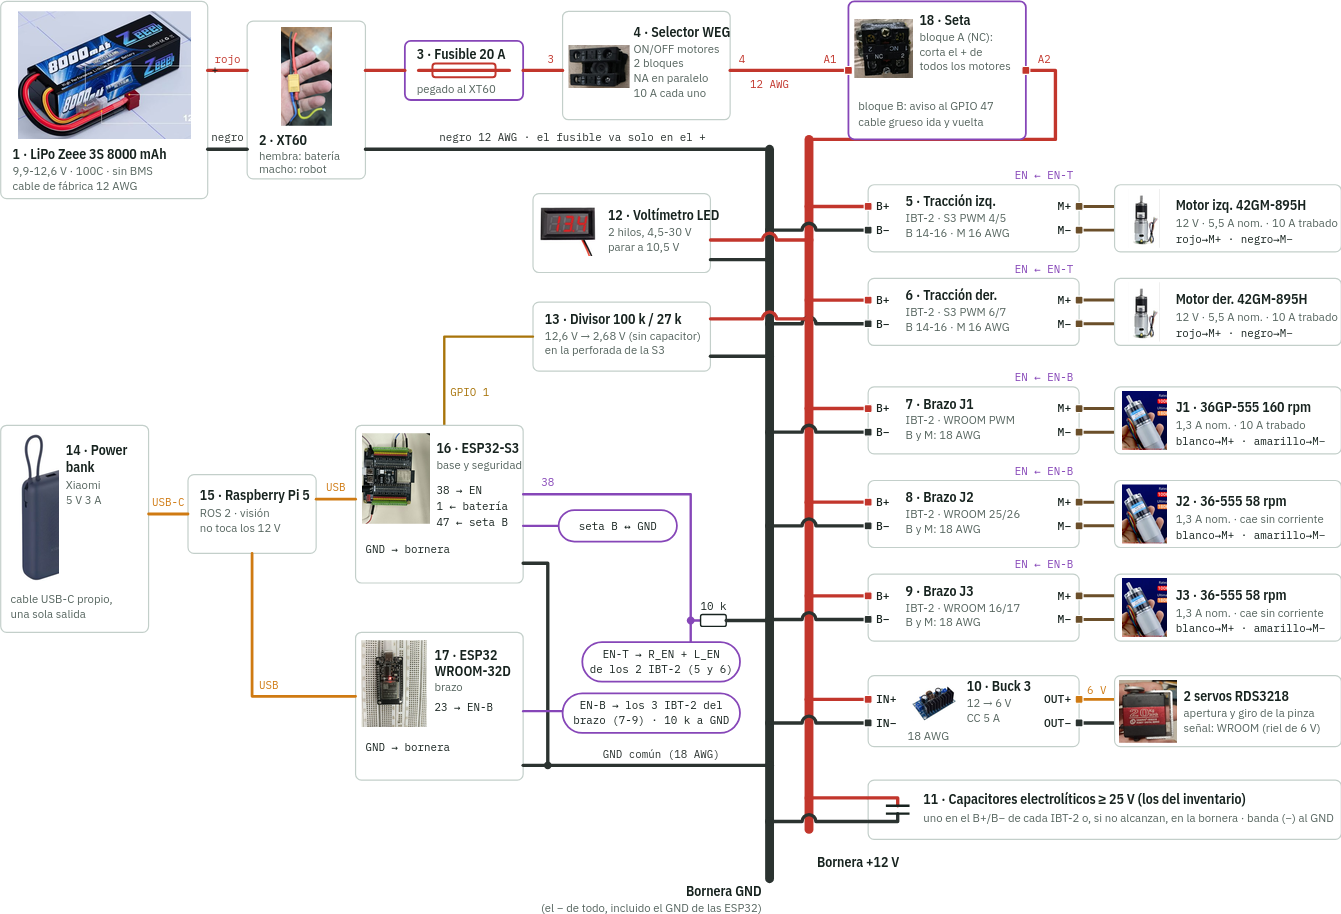
\includegraphics[width=\textwidth]{html_potencia.png}
\caption{Cableado de potencia completo, con fotos y calibres (de \archivo{docs/html/potencia.html}). Los números
coinciden con las fichas de la sección~\ref{sec:piezas}.}
\end{figure}

\section{Cada pieza}\label{sec:piezas}

\begin{figure}[H]
\centering
\begin{subfigure}{0.19\textwidth}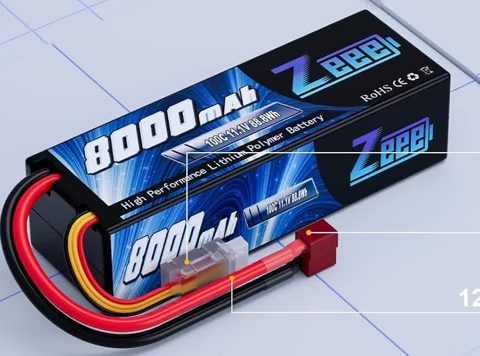
\includegraphics[width=\linewidth,height=3cm,keepaspectratio]{p_lipo.jpg}\caption{LiPo 3S}\end{subfigure}\hfill
\begin{subfigure}{0.19\textwidth}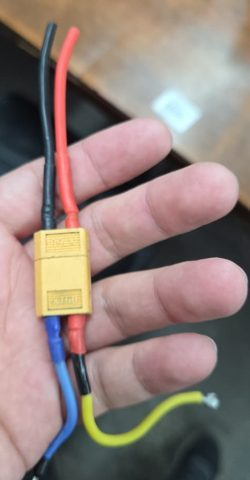
\includegraphics[width=\linewidth,height=3cm,keepaspectratio]{p_xt60.jpg}\caption{XT60}\end{subfigure}\hfill
\begin{subfigure}{0.19\textwidth}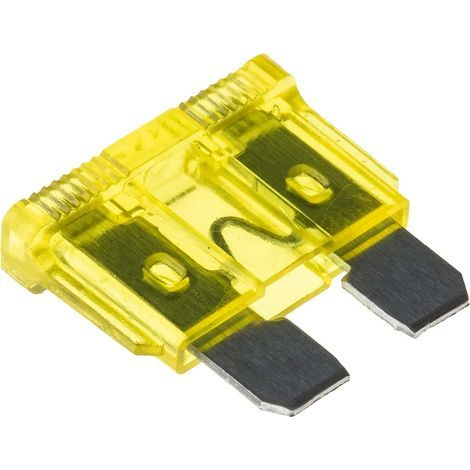
\includegraphics[width=\linewidth,height=3cm,keepaspectratio]{fusible.jpg}\caption{Fusible 20 A}\end{subfigure}\hfill
\begin{subfigure}{0.19\textwidth}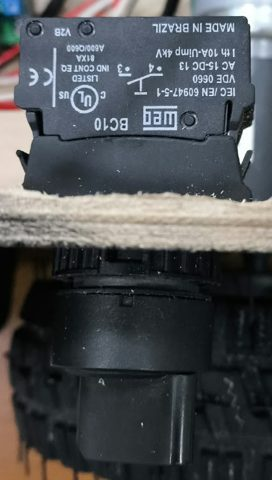
\includegraphics[width=\linewidth,height=3cm,keepaspectratio]{p_selector.jpg}\caption{Selector WEG}\end{subfigure}\hfill
\begin{subfigure}{0.19\textwidth}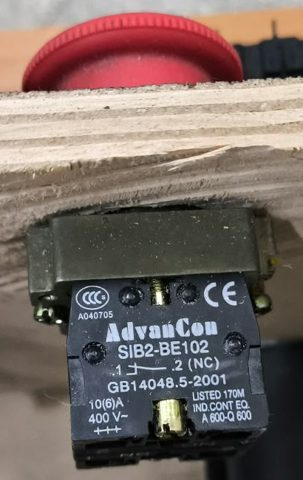
\includegraphics[width=\linewidth,height=3cm,keepaspectratio]{p_seta.jpg}\caption{Seta}\end{subfigure}\\[4pt]
\begin{subfigure}{0.19\textwidth}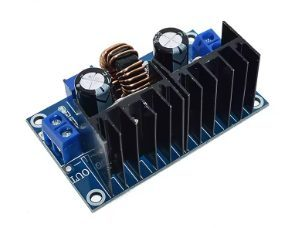
\includegraphics[width=\linewidth,height=3cm,keepaspectratio]{p_buck3.jpg}\caption{Buck 3}\end{subfigure}\hfill
\begin{subfigure}{0.19\textwidth}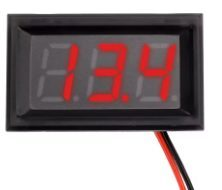
\includegraphics[width=\linewidth,height=3cm,keepaspectratio]{p_voltimetro.jpg}\caption{Voltímetro}\end{subfigure}\hfill
\begin{subfigure}{0.19\textwidth}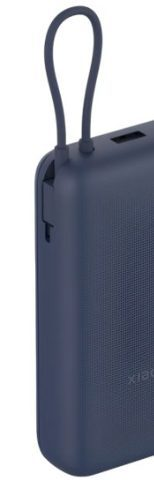
\includegraphics[width=\linewidth,height=3cm,keepaspectratio]{p_powerbank.jpg}\caption{Power bank}\end{subfigure}\hfill
\begin{subfigure}{0.19\textwidth}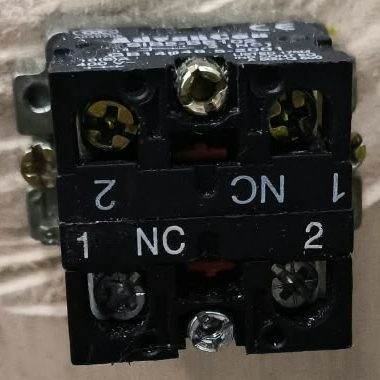
\includegraphics[width=\linewidth,height=3cm,keepaspectratio]{p_hongo_atras.jpg}\caption{Seta, atrás}\end{subfigure}\hfill
\begin{subfigure}{0.19\textwidth}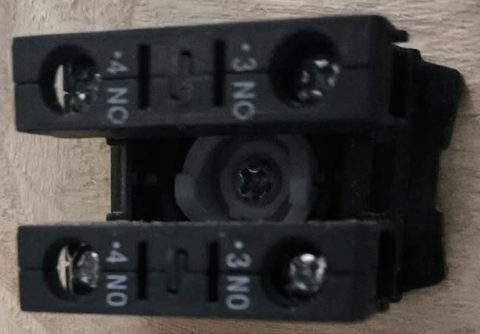
\includegraphics[width=\linewidth,height=3cm,keepaspectratio]{p_selector_atras.jpg}\caption{Selector, atrás}\end{subfigure}
\caption{Las piezas del circuito de potencia.}
\end{figure}

\begin{longtable}{@{}p{3.3cm} p{12.2cm}@{}}
\toprule
\textbf{Pieza} & \textbf{Qué hace y cómo se usa} \\
\midrule
\endhead
LiPo Zeee 3S & 11,1~V, 8000~mAh, 100C, 493~g. \textbf{No tiene BMS}: nada la protege de la sobredescarga. Se carga
  solo con el cargador balanceador y fuera del robot. Guardada varios días, a $\sim$11,4~V (3,8~V por celda). Su
  conector Deans de fábrica se cambia por un \textbf{XT60} (no hay Deans hembra). \\
XT60 & Conector de la batería. Se enchufa \textbf{con el selector en OFF} y respetando la polaridad: los IBT-2 al
  revés se rompen. Al cambiar el Deans, cortar \textbf{de a un cable} (los dos juntos con la pinza hacen un corto). \\
Fusible de auto 20~A & Lámina ATO/ATC, apto para continua hasta 32~V. Va \textbf{pegado al XT60}: el cable antes
  del fusible no está protegido. \textbf{Protege contra cortocircuitos}; no salta con dos motores trabados
  ($2 \times 10$~A es justo su nominal). Cable del bus de al menos 14~AWG. \\
Selector WEG & ON/OFF diario de los motores. Dos bloques BC10 normalmente abiertos en paralelo. \textbf{Moverlo solo
  con los motores quietos}: dos contactos en paralelo no suman 20~A al abrir (el último en separarse corta todo). \\
Seta (bloque A) & Contacto normalmente cerrado en serie con el + del bus de 12~V, después del selector. Al apretarla,
  los cinco IBT-2 y el buck quedan sin tensión. Los motores quedan en rueda libre: \textbf{no frena}. Está pensada
  para alterna (\cod{10(6)A 400V\textasciitilde}): solo para emergencias. \\
Seta (bloque B) & Otro contacto NC del mismo botón, entre el GPIO~47 de la S3 y GND. Avisa al firmware. \textbf{Nunca
  12~V en este bloque}: queman el GPIO. \\
IBT-2 (×5) & Puentes H BTS7960: 2 de tracción y 3 del brazo. Entrada de potencia B+/B−, salida al motor M+/M−. \\
Buck 3 & XL4016 (4--38~V de entrada, 5~A). Baja 12~V a 6~V para los servos, con límite de corriente en 5~A.
  \textbf{Ajustarlo sin carga y con el multímetro} antes de conectar los servos. \\
Capacitores & Electrolíticos de $\geq 25$~V cerca de los IBT-2, para absorber picos. \\
Divisor 100~k / 30~k & Baja 12,6~V a 2,91~V para el ADC del GPIO~1 de la S3. Si alguna vez vuelve la batería 10S
  (36~V), \textbf{cambiarlo antes a 120~k / 8,2~k}: con 42~V el de 30~k pondría $\sim$9~V en el GPIO y lo quema. \\
Voltímetro / indicador & Muestra la tensión a la vista. Parar a 10,5~V. \\
Power bank & 20\,000~mAh, 5~V 3~A. Una sola salida, cable incorporado (corto), arriba al lado de la Pi. No cargarlo
  mientras alimenta la Pi (puede cortar un instante). \\
\bottomrule
\end{longtable}

\section{Consumo y autonomía}

\begin{center}
\begin{tabular}{@{}lr@{}}
\toprule
\textbf{Carga} & \textbf{Potencia} \\
\midrule
Tracción avanzando a 0,25~m/s ($2 \times 60\% \times 12\text{ V} \times 3\text{ A}$) & $\sim$43~W \\
Tracción girando o en terreno malo & $\sim$70~W \\
Brazo moviéndose (J1--J3 + servos) & $\sim$26~W \\
Brazo quieto sosteniendo (J2/J3 contra el peso + pinza) & $\sim$6~W \\
Lógica: Pi 5 con YOLO ($\sim$9~W), ESP32 (0,8~W), sensores (0,6~W) & $\sim$11~W \\
\bottomrule
\end{tabular}
\end{center}

Ciclo de cosecha de un limón (60~s): 20~s avanzando, 5~s maniobrando, 25~s con el brazo en movimiento y 10~s con el
brazo quieto:
\[
P_\text{motores} = \frac{20\,(43 + 6) + 5\,(70 + 6) + 25 \cdot 26 + 10 \cdot 6}{60} \approx 34{,}5\text{ W}
\]
Con el 80~\% de la energía nominal como útil (71~Wh):

\begin{figure}[H]
\centering
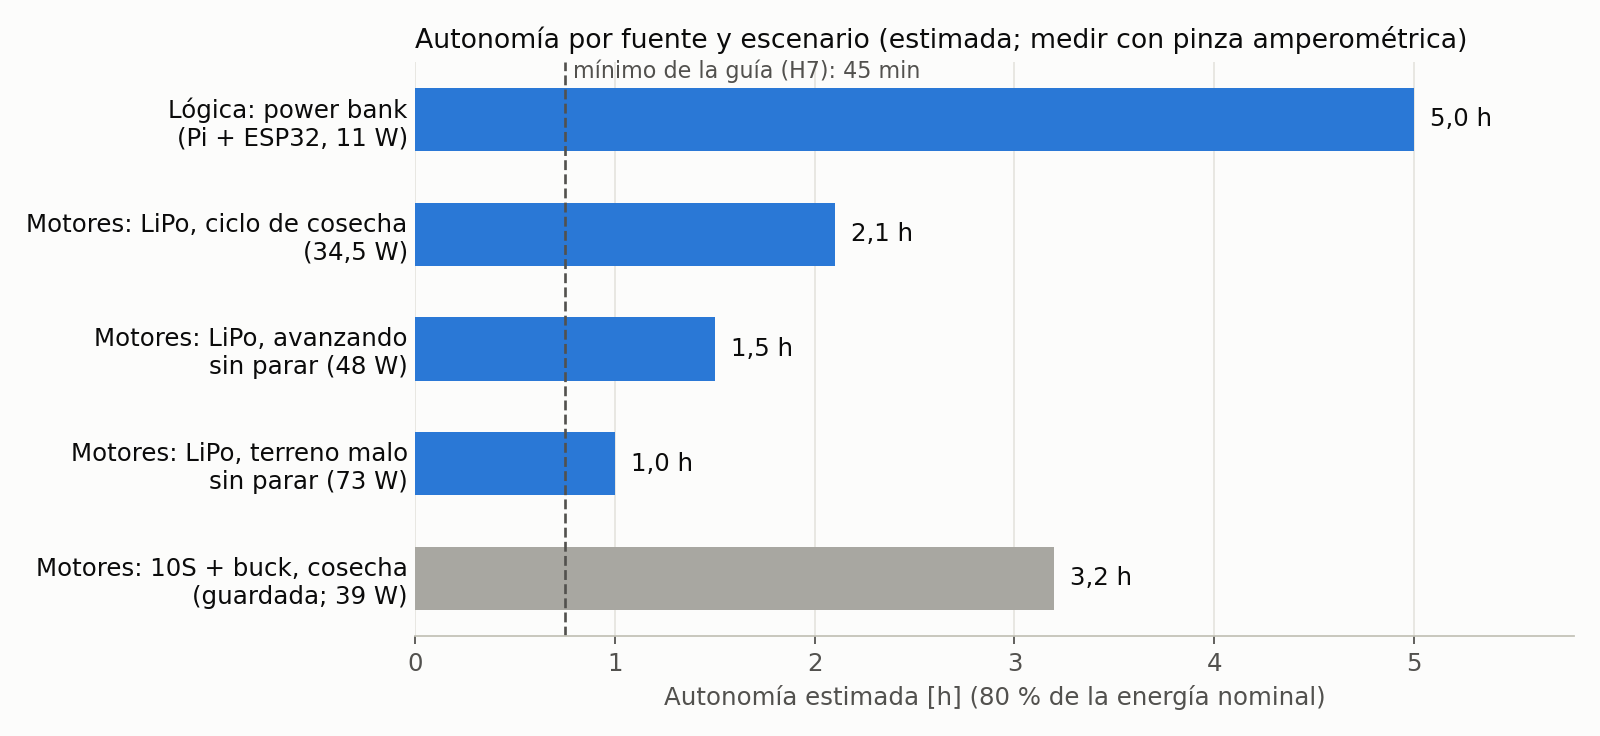
\includegraphics[width=0.85\textwidth]{autonomia.png}
\caption{Autonomía estimada por fuente y escenario (de la entrega R2~E4). La guía pide al menos 45~min. El robot
dura lo que dura la LiPo: $\sim$2,1~h de cosecha.}
\end{figure}

\section{La batería sin BMS}

\begin{peligro}[La LiPo no se protege sola]
\begin{itemize}[leftmargin=*]
  \item El firmware de la base mide la tensión y avisa \cod{BATERIA\_BAJA} a 10,5~V en \topic{/base/estado}, pero
        \textbf{no frena}: hay que parar a mano.
  \item 10,5~V en total no garantizan 3,5~V en cada celda. Ni el ADC ni el indicador ven una celda desbalanceada.
        \textbf{Medir cada celda} con el balanceador o el tester antes y después de cada prueba.
  \item Calibrar la lectura del ADC contra el tester.
  \item Con la seta apretada, el divisor marca 0~V (\cod{BATERIA\_BAJA}): es normal.
\end{itemize}
\end{peligro}

\section{Reglas para las pruebas}

La revisión de Codex del 14/10 confirmó que el conexionado está bien, pero que varios componentes no tienen
garantizado cortar con carga en continua. Por eso las pruebas son \textbf{acotadas y vigiladas}:

\begin{enumerate}
  \item Mover el selector \textbf{solo con los motores quietos}.
  \item Si se aprieta la seta, \textbf{mandar \cod{desarmar} al brazo y confirmar que quedó desarmado antes de
        soltarla} (aunque \cod{mision} esté corriendo).
  \item \textbf{Nada de pruebas de motores trabados con la LiPo}: el fusible no salta con eso. Usar una fuente
        limitada en corriente.
  \item Cables a las borneras con \textbf{cobre pelado y retorcido, sin estañar}: el estaño cede bajo el tornillo.
  \item Siempre alguien con la mano en la seta o en el selector.
  \item Apagar los 12~V antes de flashear o resetear un ESP32 (al reiniciar, los pines quedan un instante sin
        control).
\end{enumerate}
